\documentclass[12pt, openany]{report}
\usepackage[utf8]{inputenc}
\usepackage[T1]{fontenc}
\usepackage{amsmath,amsfonts,amssymb}
\usepackage{amssymb}
\usepackage{multicol}
\usepackage[a4paper,left=2.5cm,right=2.5cm,top=2.5cm,bottom=2.5cm]{geometry}
\usepackage[english]{babel}
\usepackage{libertine}
\usepackage{graphicx}
\usepackage{wrapfig}
\usepackage{algorithm}
\usepackage{algpseudocode}
\usepackage{float}
\usepackage{enumitem}
\usepackage{pythonhighlight}
\usepackage[]{titletoc}
\usepackage{empheq}
\usepackage{titlesec}
\usepackage{mathpazo}
\usepackage{xfrac}
\usepackage{textcomp}
\usepackage{mathtools}
\usepackage{caption}
\usepackage{tabularray}
\usepackage{subcaption}
\usepackage{cancel}
\usepackage[bottom]{footmisc}
\usepackage{pdfpages}
\usepackage{tabularx}
\usepackage{amsthm}
\usepackage[skins]{tcolorbox}
\titleformat{\chapter}[display]
  {\normalfont\bfseries}{}{0pt}{\Huge}
\usepackage{hyperref}
\newcommand{\hsp}{\hspace{20pt}}
\newcommand{\HRule}{\rule{\linewidth}{0.5mm}}
\newcommand{\R}{\mathbb{R}}
\newcommand{\C}{\mathcal{C}}
\newcommand{\N}{\mathbb{N}}
\renewcommand{\O}{\mathcal{O}}
\theoremstyle{definition}
\newtheorem{thm}{Theorem}[chapter]
\newtheorem{definition}[thm]{Definition}
\newtheorem{lem}[thm]{Lemma}

\hbadness=100000
\begin{document}
\begin{titlepage}
    \begin{sffamily}
    \begin{center}
        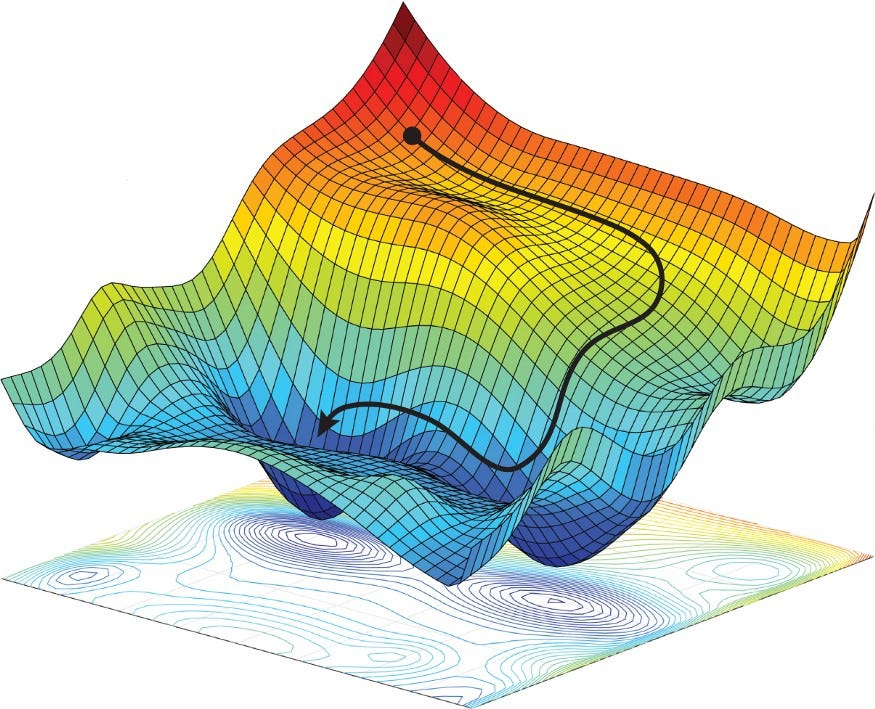
\includegraphics[scale=0.3]{img/page_de_garde.png} \\[1cm]
        \HRule \\[0.4cm]
        { \huge \bfseries LINMA2460 Nonlinear Programming \\[0.4cm] }
    
        \HRule \\[1.5cm]
        \textsc{\LARGE Simon Desmidt\\ Issambre L'Hermite Dumont}\\[1cm]
        \vfill
        \vspace{2cm}
        {\large Academic year 2024-2025 - Q2}
        \vspace{0.4cm}
         
        
\includegraphics[width=0.15\textwidth]{img/epl.png}
        
        UCLouvain\\
    
    \end{center}
    \end{sffamily}
\end{titlepage}

\setcounter{tocdepth}{1}
\tableofcontents
\chapter{Definitions, notations and random properties}
\begin{itemize}
	\item The Taylor expansion of order $p$ of the function $f$ around $x_k$ and evaluated at $y$ is: 
	\begin{equation}
		T_p(y;x_k) = f(x_k) + \sum_{i=1}^{p} \frac{1}{i!} D^i f(x_k) (y-x_k)^i
	\end{equation}
	\item We can thus define the gradient w.r.t. $y$ of the Taylor expansion of order $p$ of $f$ around $x_k$ and evaluated at $x_{k+1}$:
	\begin{equation}
		\nabla_y T_p(x_{k+1};x_k) = \left. \nabla_y T_p(y;x_k) \right|_{y=x_{k+1}}
	\end{equation}
	\item An oracle is a "black box" that gives information about the derivatives based on $x$. The general form of an oracle is:
	\begin{equation}
		\text{p-order oracle:} \quad x \mapsto \{D^if(x)\}_{i=0}^p
	\end{equation}
	And so we have the following simple oracles examples:
	\begin{equation}
		\begin{aligned}
			\text{Zero}^{th} \text{-order oracle:} \quad &x \mapsto \{f(x)\} \\
			\text{First-order oracle:} \quad &x \mapsto \{ f(x), \nabla f(x) \} \\
			\text{Second-order oracle:} \quad &x \mapsto \{ f(x), \nabla f(x), \nabla^2 f(x) \}
		\end{aligned}
	\end{equation}
    \item $\C^p_L(\R^n)$: Class of functions p-times continuously differentiable with L-Lipschitz continuous p-order derivative, i.e. $\| D^pf(x) - D^pf(y) \| \leq L \|x-y \|$, $\forall x,y\in \R^n$. And so we have the following simple classes of problems:
    \begin{itemize}
		\item $\C^1_L(\R^n)$: Class of continuously differentiable functions with L-Lipschitz gradient;
    \item $\C^2_L(\R^n)$: Class of continuously differentiable functions with L-Lipschitz hessian.
	\end{itemize}
	\item  pth-order method (generalization of GM):
	\begin{equation}
		x_{k+1} = \arg\min_{y\in \R^n} \Omega_{x_k,y,p}(y) \equiv T_{x_k,p}(y) + \frac{M}{(p+1)!}\|y-x_k\|^{p+1}
	\end{equation}
	\item Convergence rate: 
	\begin{itemize}
		\item Linear:
		\begin{equation}\label{eq:linear_convergence_rate}
			\|x_{k+1}-x^*\| \leq \alpha \|x_k-x^*\| \quad \forall k\geq 0, \alpha \in (0,1)
		\end{equation}
		\item Super Linear:
		\begin{equation}\label{eq:super_linear_convergence_rate}
			\lim_{k \to +\infty} \frac{\|x_{k+1}-x^*\|}{\|x_k-x^*\|} = 0
		\end{equation}
		\item Quadratic:
		\begin{equation}\label{eq:quadratic_convergence_rate}
			\|x_{k+1}-x^*\| \leq \beta \|x_k-x^*\|^2 \quad \forall k\geq 0, \beta > 0
		\end{equation}
	\end{itemize}
\end{itemize}
\section{Properties}
\begin{itemize}
	\item For a function $f\in \C^1(\Omega)$ and $\Omega$ is bounded, the following holds: $\lVert \nabla f(x)\rVert \le L$ for all $x\in \Omega$ for some $L\ge 0$.
	\item By the mean value theorem, for a continuously differentiable function $f$, $\forall x,y\in \Omega,\: \exists \ z\in \Omega:$ $f(y)-f(x) = \langle \nabla f(z),y-x\rangle$.
	\item For a matrix $A$ and a scalar $b$, $\lVert A\rVert \le b\Longrightarrow |\lambda (A)|\le b \Longrightarrow |A| \preceq bI_n$, where the absolute value of the matrix is taken component wise. 
\end{itemize}
\section{Complexity table}
\begin{center}
	\begin{tabular}{|c|c|c|c|c|c|}
		\hline
		Method & Lipschitz & $\nabla f$ & $\nabla^2 f$ & \dots & $\nabla^p f$ \\
		\hline
		Zero order & & $O(n\varepsilon^{-2})$ & & & \\
		\hline
		First order & $p=1$ & $O(\varepsilon^{-2})$ & & & \\
		\hline
		Second order & $p=2$ & \textcolor{red}{\cancel{X}} & $O(\varepsilon^{-3/2})$ & & \\
		\hline
		\vdots & & \textcolor{red}{\cancel{X}} & \textcolor{red}{\cancel{X}} & $\ddots$ & \\
		\hline
		p order & & \textcolor{red}{\cancel{X}} & \textcolor{red}{\cancel{X}} & \textcolor{red}{\cancel{X}} & $O(\varepsilon^{-\frac{p+1}{p}})$ \\
		\hline
	\end{tabular}
\end{center}
\section{GM VS Newton: table}
\begin{center}
	\begin{tabular}{|c|c|c|c|}
		\hline
		& cost per iteration & cost of memory & Local rate\\
		\hline
		GM & $\O (n)$ & $\O (n)$ & Linear\\
		\hline
		Quasi-Newton & $\O (n^2)$ & $\O (n^2)$ & Super Linear\\
		\hline
		Newton & $\O (n^3)$ & $\O (n^2)$ & Quadratic\\
		\hline
	\end{tabular}
\end{center}
\begin{itemize}
	\item [$\rightarrow$] For the GM, we assume that we don't need to compute the gradient at each iteration.
\end{itemize}
\chapter{TODO}\label{chap:right_oracle}
We can generalise the property of a L-Lipschitz function to $f\in \C_L^p(\R^n)$. For $p=1$, we had 
\begin{equation}
	f(y)\le f(x_k) + \langle \nabla f(x_k),y-x_k\rangle + \frac{L}{2}\lVert y-x_k\rVert^2 \qquad \forall y\in \R^n 
\end{equation}
For a general value of $p$, it becomes 
\begin{equation}
	f(y) \le T_p(y;x_k) + \frac{L}{(p+1)!}\lVert y-x_k\rVert^{p+1} \qquad \forall y\in \R^n 
\end{equation}
Using this, \textcolor{blue}{we need a $p$-th order oracle} for the method to work. \\
To solve $\min_{x\in \R^n} f(x)$, we can use the iteration 
\begin{equation}\label{eq:argmin}
	x_{k+1} = \arg\min_{y\in \R^n} T_p(y;x_k)+\frac{M}{(p+1)!}\lVert y-x_k\rVert^{p+1}
\end{equation}
where the constant $M$ is an approximation of the Lipschitz constant $L$. \textcolor{blue}{Assuming $f\in \C^p_L(\R^n)$}, we have 
\begin{equation}
	\begin{aligned}
		f(x_{k+1}) &\le T_p(x_{k+1};x_k) + \frac{L}{(p+1)!}\lVert x_{k+1}-x_k\rVert^{p+1}\\
		&= \underbrace{T_p(x_{k+1};x_k) + \frac{M}{(p+1)!}\lVert x_{k+1}-x_k\rVert^{p+1}}_{\le f(x_k)} + \frac{(L-M)}{(p+1)!}\lVert x_{k+1}-x_k\rVert^{p+1}
	\end{aligned}
\end{equation}
where the inequality $\le f(x_k)$ is due to the decrease of $f$ and equation \eqref{eq:argmin}. 
\textcolor{blue}{Suppose that $M>2L$}. After some algebraic manipulations, we get
\begin{equation}\label{eq:bound}
	f(x_k)-f(x_{k+1}) \ge \frac{L}{(p+1)!}\lVert x_{k+1}-x_k\rVert^{p+1}
\end{equation}
On the other hand, using the triangular inequality, 
\begin{equation}
	\begin{aligned}
		\lVert \nabla f(x_{k+1})\rVert & \le \lVert \nabla f(x_{k+1})-\nabla_y T_p(x_{k+1};x_k)\lVert\\
		& + \underbrace{\left \lVert \nabla_y T_p(x_{k+1};x_k)+\nabla \left.\left(\frac{M}{(p+1)!} \lVert \cdot -x_k\rVert^{p+1}\right)\right|_{y=x_{k+1}}\right \rVert}_{=0}	\\
		& + \left\lVert \nabla \left.\left(\frac{M}{(p+1)!}\lVert \cdot -x_k\rVert^{p+1}\right)\right|_{y=x_{k+1}}\right \rVert \\
		& \le \frac{L}{p!}\lVert x_{k+1}-x_k\rVert^p + \frac{M}{p!} \lVert x_{k+1}-x_k\rVert^p
	\end{aligned}
\end{equation}
\begin{equation}\label{eq:bound_on_x}
	\Longrightarrow \lVert x_{k+1}-x_k\rVert \ge \left(\frac{p!}{L+M}\right)^{1/p}\lVert \nabla f(x_{k+1})\rVert^{1/p}
\end{equation}
Combining equations \eqref{eq:bound} and \eqref{eq:bound_on_x}, 
\begin{equation}\label{eq:next_bound}
	f(x_k)-f(x_{k+1}) \ge \underbrace{\frac{L}{(p+1)!}\left(\frac{p!}{L+M}\right)^{\frac{p+1}{p}}}_{\eqcolon C(L)} \lVert \nabla f(x_{k+1})\rVert^{\frac{p+1}{p}}
\end{equation}
Let $T(\varepsilon) = \inf \{k\in \mathbb{N}:\: \lVert \nabla f(x_k)\rVert\le \varepsilon\}$. \textcolor{blue}{Assume that $T(\varepsilon)\ge 2$ and $f(x)\ge f_{low}$ $\forall x\in \R^n$.} Summing up \eqref{eq:next_bound} for $k=0,\dots, T(\varepsilon)-2$,
\begin{equation}
	\begin{aligned}
		f(x_0)-f_{low} &\ge f(x_0)-f(x_{T(\varepsilon)-1}) = \sum_{k=0}^{T(\varepsilon)-2} f(x_k)-f(x_{k+1}) \\ 
		& \ge (T(\varepsilon)-1)C(L) \varepsilon^{\frac{p+1}{p}}\\
		\Longrightarrow T(\varepsilon) &\le 1 + \frac{f(x_0)-f_{low}}{C(L)} \varepsilon^{-\frac{p+1}{p}} \equiv \O\left(\varepsilon^{-\frac{p+1}{p}}\right)
	\end{aligned}
\end{equation}
\chapter{Gradient descent without gradient}\label{chap:}
For this problem consider an adversarial attack on block-based image classifier. We have a machine learning model that given an image $a\in\R^p$ it returns $c(a)\in\R^m$, where $c_j(a) \in [0,1]$ is the probability of image $a$ to be in class $j$. The classifier prediction is: $j(a) = \arg\max_{j\in [1,\dots,m]} c_j(a)$.\\
\textcolor{red}{TODO - Add mise en situation ou pas?}
\newline

Given $x_k$ let us decide:
\begin{equation}
	x_{k+1} = x_k - \frac{1}{\sigma} g_{h_k}(x_k) \quad \quad \quad h_k > 0, \: \sigma > 0
\end{equation}
where $g_{h_k}(x_k) \in \R^n$ is given by:
\begin{equation}
	[g_{h_k}(x_k)]_j = \frac{f(x_k+he_j)-f(x_k)}{h_k} \quad \quad \quad \forall j\in [1,\dots,m]
\end{equation}
\textcolor{blue}{Suppose that $f\in \C^1_L(\R^n)$}. Then,
\begin{equation}
	\|\nabla f(x_k) - g_{h_k}(x_k)\| \leq \frac{L \sqrt{n}}{2} h_k
\end{equation}
Thus 
\begin{equation}
	\begin{aligned}
		f(x_{k+1}) &\leq f(x_k) &&+ \langle \nabla f(x_k), x_{k+1}-x_k\rangle + \frac{L}{2}\lVert x_{k+1}-x_k\rVert^2\\
		&= f(x_k) &&+ \langle g_{h_k}(x_k), x_{k+1}-x_k\rangle + \frac{\sigma}{2} \|x_{k+1}-x_k\|\\
		& &&+ \langle \nabla f(x_k) - g_{h_k}(x_k), x_{k+1}-x_k\rangle + \frac{(L-\sigma)}{2}\lVert x_{k+1}-x_k\rVert^2\\
		&\leq f(x_k) &&- \frac{1}{\sigma} \|g_{h_k}(x_k)\|^2 + \frac{1}{2\sigma} \|g_{h_k}(x_k)\|^2 \\
		& &&+ \| \nabla f(x_k) - g_{h_k}(x_k)\| \frac{1}{\sigma} \|g_{h_k}(x_k)\| + \frac{(L-\sigma)}{2\sigma^2} \|g_{h_k}\|^2\\
		& \leq f(x_k) &&- \frac{1}{2\sigma} \|g_{h_k}(x_k)\|^2 + \frac{L \sqrt{n}}{2} h_k \frac{1}{\sigma} \|g_{h_k}\| + \frac{(L-\sigma)}{2\sigma^2} \|g_{h_k}\|^2\\
		&\leq f(x_k) &&- \frac{1}{2\sigma} \|g_{h_k}(x_k)\|^2 + \frac{L}{2} \left( \frac{nh_k^2}{2}+ \frac{1}{2 \sigma} \|g_{h_k}(x_k)\|^2 \right) + \frac{(L-\sigma)}{2\sigma^2} \|g_{h_k}\|^2\\
		&= f(x_k) &&- \left( \frac{2\sigma - L -2(L - \sigma)}{4 \sigma^2} \right) \|g_{h_k}(x_k)\|^2 + \frac{Ln}{4} h_k^2\\
		&= f(x_k) &&- \frac{(4\sigma -3L)}{4 \sigma} \|g_{h_k}(x_k)\|^2  + \frac{Ln}{4} h_k^2
	\end{aligned}
\end{equation}
\begin{equation}
	\Longrightarrow \frac{(4\sigma -3L)}{4 \sigma} \|g_{h_k}(x_k)\|^2 \leq f(x_k) - f(x_{k+1}) + \frac{Ln}{4} h_k^2
\end{equation}
\textcolor{blue}{If $\sigma \gg L$, then}
\begin{equation}
	\frac{1}{4\sigma} \|g_{h_k}(x_k)\|^2 \leq f(x_k) - f(x_{k+1}) + \frac{\sigma n}{4} h_k^2
\end{equation}
On the other hand, we have
\begin{equation}
	\begin{aligned}
		\|\nabla f(x_k)\| &\leq \|\nabla f(x_k) - g_{h_k}(x_k)\| + \|g_{h_k}(x_k)\|\\
		&\leq \frac{L \sqrt{n}}{2} h_k + \|g_{h_k}(x_k)\|\\
	\end{aligned}
\end{equation}
Using trick \eqref{eq:sq2} in chapter \ref{chap:tricks},
\begin{equation}
	\begin{aligned}
		\Longrightarrow \|\nabla f(x_k)\|^2 &\leq 2 \left( \frac{L \sqrt{n}}{2} h_k \right)^2 + 2 \|g_{h_k}(x_k)\|^2\\
		&\leq \frac{L^2 n}{2} h_k^2 + 2 \|g_{h_k}(x_k)\|^2 
	\end{aligned}
\end{equation}
\begin{equation}
	\Longrightarrow \frac{1}{8 \sigma} \|\nabla f(x_k)\|^2 \leq \frac{L^2n}{16\sigma} h_k^2 + \frac{1}{4\sigma} \|g_{h_k}(x_k)\|^2
\end{equation}
\begin{equation}\label{eq:brigitte}
	\Longrightarrow \frac{1}{8 \sigma} \|\nabla f(x_k)\|^2 \leq f(x_k) - f(x_{k+1}) + \frac{\sigma n}{4} h_k^2 + \frac{\sigma n}{16}h_k^2
\end{equation}
Let $T(\varepsilon) = \inf \{k\in \mathbb{N}: \|\nabla f(x_k)\| \leq \varepsilon \}$, \textcolor{blue}{with $f(x)$ bounded below by $f_{low}$}, summing up \eqref{eq:brigitte} for $k=0,\dots, T(\varepsilon)-1$:
\begin{equation}
	\frac{T(\varepsilon)}{8 \sigma} \varepsilon^2 \leq f(x_0) - f_{low} + \frac{5 \sigma n}{4} \sum_{k=0}^{T(\varepsilon)-1} h_k^2
\end{equation}
\textcolor{blue}{If $\{h_k^2\}$ is summable}
\begin{equation}
	\Longrightarrow T(\varepsilon) \leq 8 \sigma \left( f(x_0) - f_{low} + \frac{5 \sigma n}{4} \sum_{k=0}^{T(\varepsilon)-1} h_k^2\right) \varepsilon^2 = \O(\varepsilon^2)
\end{equation}
In terms of call to the oracle, we have a complexity bound of $\O(n\varepsilon^2)$.

\chapter{Local rates of convergence}
\section{Linear rate of GM}
Let \textcolor{blue}{$f \in \C_M^{2,2}(\R^n)$}. Assume \textcolor{blue}{$f$ has a local minimizer $x^*$ such that 
\begin{equation}\label{eq:hessian_bound}
	\mu I_n \preceq \nabla^2 f(x^*) \preceq MI_n
\end{equation}}
Let $x_{k+1} = x_k - \frac{1}{L} \nabla f(x_k)$ for a given $x_0 \in \R^n$.\\
Notice that
\begin{equation}\label{eq:G_k}
	\begin{aligned}
		\nabla f(x_k) &= \nabla f(x_k) - \nabla f(x^*)\\
		&= \int_{0}^{1} \nabla^2 f(x^* + \tau(x_k-x^*)) (x_k-x^*) d\tau\\
		&= \int_{0}^{1} \nabla^2 f(x^* + \tau(x_k-x^*)) d\tau (x_k-x^*) \\
		&= G_k (x_k-x^*)
	\end{aligned}
\end{equation}
Then,
\begin{equation}
	\begin{aligned}
		\|x_{k+1} - x^*\| &= \|x_k - \frac{1}{L} \nabla f(x_k) - x^*\|\\
		&= \|(I_n-\frac{1}{L}G_k)(x_k-x^*)\|\\
		&\leq \|I_n - \frac{1}{L}G_k\| \|x_k-x^*\|
	\end{aligned}
\end{equation}
Since $f \in C_M^{2,2}(\R^n)$, we have $\|\nabla^2f(x^*+\tau(x_k-x^*))-\nabla^2f(x^*)\| \leq \tau M \|x_k -x^*\|$ and using this we get:
\begin{equation}
	|\langle \nabla^2f(x^*+\tau(x_k-x^*))-\nabla^2f(x^*) v, v\rangle| \leq \tau M \|x_k -x^*\| \|v\|^2 \quad \forall v \in \R^n
\end{equation}
Using the bound \eqref{eq:hessian_bound} and the previous inequality, we get:
\begin{equation*}
		\tau M \|x_k -x^*\| \|v\|^2 \leq |\langle \nabla^2f(x^*+\tau(x_k-x^*))-\nabla^2f(x^*) v, v\rangle| \leq \tau M \|x_k -x^*\| \|v\|^2\\
\end{equation*}
\begin{equation*}
	\nabla^2 f(x^*) - \tau M \|x_k -x^*\| I_n \preceq \nabla^2f(x^*+\tau(x_k-x^*)) \preceq \nabla^2 f(x^*) + \tau M \|x_k -x^*\|I_n 
\end{equation*}
\begin{equation*}
	(\mu - \tau M \|x_k -x^*\|)I_n \preceq \nabla^2f(x^*+\tau(x_k-x^*)) \preceq (L + \tau M \|x_k -x^*\|) I_n 
\end{equation*}
By the properties of the semi-definite matrices, and the trick \eqref{eq:vtrick}, we have:
\begin{equation}
	\begin{aligned}
		\int_{0}^{1} (\mu - \tau M \|x_k -x^*\|) \|v\|^2 d\tau &\leq \int_{0}^{1} \langle \nabla^2f(x^*+\tau(x_k-x^*)) v,v \rangle d\tau\\ 
		&\leq \int_{0}^{1} (L + \tau M \|x_k -x^*\|) \|v\|^2 d\tau \quad \forall v \in \R^n
	\end{aligned}
\end{equation}
By using $G_k$ and some constants, we get:
\begin{equation}
	-\frac{1}{L}(L+\frac{M}{2}\|x_k -x^*\|)I_n \preceq - \frac{1}{L} G_k \preceq -\frac{1}{L}(\mu - \frac{M}{2}\|x_k -x^*\|)I_n
\end{equation}
\begin{equation}
	\left(1-\frac{1}{L}(L+\frac{M}{2}\|x_k -x^*\|)\right)I_n \preceq I_n - \frac{1}{L}G_k \preceq \left(1-\frac{1}{L}(\mu - \frac{M}{2}\|x_k -x^*\|)\right)I_n
\end{equation}
And finally, we get:
\begin{equation}\label{eq:eq3cm3}
	\begin{aligned}
		\|I_n - \frac{1}{L}G_k\| &\leq \max\left\{\left|1-\frac{1}{L}(L + \frac{M}{2}\|x_k -x^*\|)\right|,\left|1-\frac{1}{L}(\mu - \frac{M}{2}\|x_k -x^*\|)\right|\right\}\\
		&= \max\left\{\frac{M}{2L}\|x_k -x^*\|, 1-\frac{\mu}{L}+\frac{M}{2L}\|x_k -x^*\|\right\}\\
		&= 1-\frac{\mu}{L}+\frac{M}{2L}\|x_k -x^*\|
	\end{aligned}
\end{equation}
\textcolor{blue}{Suppose that $\frac{M}{2L} \|x_k -x^*\| \leq \frac{\mu}{2L} \Longleftrightarrow \|x_k -x^*\| \leq \frac{\mu}{M}$}\\
Then, in \eqref{eq:eq3cm3}, we get:
\begin{equation}
	\|I_n - \frac{1}{L}G_k\| \leq 1-\frac{\mu}{2L} < 1
\end{equation}
And so, by \eqref{eq:G_k}
\begin{equation}\label{eq:bound_by_G_k}
	\|x_{k+1} - x^*\| \leq \|I_n - \frac{1}{L}G_k\| \|x_k -x^*\| < \|x_k -x^*\|
\end{equation}
If $\|x_0 - x^* \|< \frac{\mu}{M}$, it follows from the previous reasoning that:
\begin{equation}
	\|x_2 - x^*\| \leq  (1-\frac{\mu}{2L}) \|x_1-x^*\| \leq (1-\frac{\mu}{2L})^2 \|x_0-x^*\|\leq \frac{\mu}{M}
\end{equation} 
And so by induction, we can conclude that:
\begin{equation}\label{eq:bound_x_k_induction}
	\|x_k - x^*\| \leq \left(1-\frac{\mu}{2L}\right)^k \|x_0-x^*\| \quad \forall k \geq 0
\end{equation}
\begin{center}
	\color{red}\boxed{\textcolor{black}{\Rightarrow \text{Linear rate of convergence}}}\color{black}\\
\end{center}

Given $\varepsilon > 0$, let $T(\varepsilon) = \inf\{k\in \mathbb{N} : \|x_k -x^*\|\leq \varepsilon\}$. Then, if $T(\varepsilon) \geq 1$ and using \eqref{eq:bound_x_k_induction}, we get:
\begin{equation}
	\begin{aligned}
		\varepsilon < \|x_{T(\varepsilon)-1} - x^*\| &\leq \left(1-\frac{\mu}{2L}\right)^{T(\varepsilon)-1} \|x_0 - x^*\|\\
		\log \left(\frac{\varepsilon}{\|x_0 - x^*\|}\right) &\leq (T(\varepsilon)-1) \log \left(1-\frac{\mu}{2L}\right)\\
		T(\varepsilon)-1 &\leq \frac{\log \left(\frac{\varepsilon}{\|x_0 - x^*\|}\right)}{\log \left(1-\frac{\mu}{2L}\right)} = \frac{\log \left(\|x_0 - x^*\|\varepsilon^{-1}\right)}{|\log \left(1-\frac{\mu}{2L}\right)|}
	\end{aligned}
\end{equation}
\begin{center}
	\color{red}
	\boxed{\color{black} T(\varepsilon) \leq \mathcal{O}(\log(\varepsilon^{-1})) }
	\color{black}\\
\end{center}
\begin{itemize}
	\item [$\rightarrow$] Note: convexity was never assumed!
\end{itemize}

\section{Local quadratic convergence of Newton's method}
\textcolor{blue}{Let $f \in \C_M^{2,2}(\R^n)$. Assume $f$ has a local minimizer $x^*$ such that
\begin{equation}\label{eq:hessian_bound2}
	\mu I_n \preceq \nabla^2 f(x^*) \quad \mu > 0
\end{equation}}
Given $x_0 \in \R^n$, let:
\begin{equation}\label{eq:newton}
	x_{k+1} = x_k - \nabla^{-2} f(x_k) \nabla f(x_k)
\end{equation}
We have, by the previous equation and the definition of $G_k$ \eqref{eq:G_k}:
\begin{equation}\label{eq:bound_x_k+1}
	\begin{aligned}
		\|x_{k+1}-x^*\| &= \|x_k - \nabla^{-2} f(x_k) \nabla f(x_k) - x^*\|\\
		&= \|(x_k-x^*)-\nabla^{-2} f(x_k)G_k(x_k-x^*)\|\\
		&= \|\nabla^{-2} f(x_k) \left(\nabla^2f(x_k)-\int_{0}^{1}\nabla^2f(x^*+\tau(x_k-x^*))d\tau\right)(x_k-x^*)\|\\
		&= \|\nabla^{-2} f(x_k) \left( \int_{0}^{1} \nabla^2f(x_k)-\nabla^2f(x^*+\tau(x_k-x^*))d\tau\right)(x_k-x^*)\|\\
		&\leq \|\nabla^{-2} f(x_k)\| \left( \int_{0}^{1} \left\|\nabla^2f(x_k)-\nabla^2f(x^*+\tau(x_k-x^*))\right\|d\tau\right)\|x_k-x^*\|\\
		&\leq \|\nabla^{-2} f(x_k)\| \left( \int_{0}^{1} M(1-\tau) \|x_k-x^*\|d\tau\right)\|x_k-x^*\|\\
		&\leq \|\nabla^{-2} f(x_k)\|\|x_k-x^*\|^2\frac{M}{2}
	\end{aligned}
\end{equation}
Since $f\in \C^{2,2}_M(\R^n)$, we have
\begin{equation}
	\nabla^2 f(x^*+\tau(x_k-x^*)) - \nabla^2 f(x^*) \succeq \tau M \|x_k-x^*\|I_n
\end{equation}
\begin{equation}
	\begin{aligned}
		\nabla^2 f(x_k) &\succeq \nabla^2 f(x^*) - M \|x_k-x^*\|I_n\\
		&\succeq (\mu - M \|x_k-x^*\|)I_n\\
		\lambda_{\min}(\nabla^2 f(x_k)) &\geq \mu - M \|x_k-x^*\|
	\end{aligned}
\end{equation}
Suppose that $-M \|x_k-x^*\| \geq - \frac{\mu}{2} \Leftrightarrow \|x_k-x^*\| \leq \frac{\mu}{2M}$\\
Then,
\begin{equation}
	\begin{aligned}
		\lambda_{\min}(\nabla^2 f(x_k)) &\geq \frac{\mu}{2}\\
		\lambda_{\max}(\nabla^{-2} f(x_k)) &\leq \frac{2}{\mu}\\
		\Rightarrow \|\nabla^{-2} f(x_k)\| &\leq \frac{2}{\mu}
	\end{aligned}
\end{equation}
Therefore, by \eqref{eq:bound_x_k+1}, we conclude that:
\begin{equation}
	\begin{aligned}
		\|x_{k+1}-x^*\| &\leq \frac{M}{2}\|\nabla^{-2}f(x_k)\|\|x_k-x^*\|\\
		&\leq \frac{M}{\mu}\|x_k-x^*\|^2
	\end{aligned}
\end{equation}
If $\|x_k-x^*\| \leq \frac{\mu}{2M}$ then,
\begin{equation}\label{eq:bound_of_x_k1_by_x_k}
	\|x_{k+1}-x^*\| \leq \frac{M}{\mu} \|x_k - x^*\|^2 = \frac{1}{2} \|x_k - x^*\|
\end{equation}
If $\|x_0-x^*\| \leq \frac{\mu}{2M}$ then $\{x\}_{k\geq0} \subset B[x^*,\frac{\mu}{2M}]$.\\
Denote $\delta_k = \frac{M}{\mu} \|x_k-x^*\|$, then we have $\delta_0 = \frac{M}{\mu} \|x_0-x^*\| \leq \frac{1}{2}$, and if we combine this with \eqref{eq:bound_of_x_k1_by_x_k}, we get:
\begin{equation}
	\delta_{k+1} \leq \delta_k^2 \quad \forall k \geq 0
\end{equation}
And if we proceed by recurcence, we get:
\begin{equation}
	\begin{aligned}
		\delta_1 \leq &\delta_0^2 \leq \left(\frac{1}{2}\right)^2\\
		\delta_2 \leq &\delta_1^2 \leq \left(\frac{1}{2}\right)^4\\
		&\vdots\\
		&\delta_k \leq \left(\frac{1}{2}\right)^{2^k} \quad \forall k \geq 0
	\end{aligned}
\end{equation}
\begin{equation}\label{eq:quadratic_rate_of_convergence}
	\Rightarrow \|x_k-x^*\|\leq \frac{\mu}{M} \left(\frac{1}{2}\right)^{2^k}
\end{equation}
Let $T(\varepsilon) = \inf\{k\in\N: \|x_k-x^*\|\leq \varepsilon\}$ and suppose that $T(\varepsilon) \geq 1$. Then using the convergence rate \eqref{eq:quadratic_rate_of_convergence}, we can state the maximal number of iterations:
\begin{equation}
	\varepsilon \leq \|x_{T(\varepsilon)-1}-x^*\| \leq \frac{\mu}{M} \left(\frac{1}{2}\right)^{2^{T(\varepsilon)-1}}
\end{equation}
\begin{equation}
	2^{2^{T(\varepsilon)-1}} \leq \frac{\mu}{M} \varepsilon^{-1}
\end{equation}
\color{red}
\boxed{\color{black} \Rightarrow T(\varepsilon) \leq \log_2(\log_2(\frac{\mu}{M} \varepsilon^{-1}))}
\color{black}

\section{Quasi Newton methods}
\subsection{SR1 Update}
One step of a Quasi-Newton method is given by:
\begin{equation}\label{eq:quasi_newton}
	x_{k+1} = x_k -B_k \nabla f(x_k)
\end{equation}
With $B_k \in \R^{n\times n}$, symmetric and non-singular\\
Suppose that $x_k \to x^*$ when $k \to \infty$, and that $\nabla^2f(x_k) \succeq \mu I_n$ with $\mu \geq 0$\\
We want the condition on $B_k$ to have a Super Linear convergence \eqref{eq:super_linear_convergence_rate} of the Quasi-Newton method. So lets assume that $f \in \C_M^{2,2}(\R^n)$.\\
Then,
\begin{equation}\label{eq:bound_hessian_difference}
	\|\nabla^2f(x_{k+1}-\nabla^2f(x_k))\| \leq M \|x_{k+1}-x_k\|
\end{equation}
\textcolor{red}{GOOD LABEL ?}
\begin{equation}\label{eq:M_smoothness}
	\|\nabla f(x_{k+1}-\nabla f(x_k)-\nabla^2 f(x_k)(x_{k+1}-x_k))\| \leq \frac{M}{2} \|x_{k+1}-x_k\|^2
\end{equation}
Therefore
\begin{equation}
	\begin{aligned}
		\nabla f(x_{k+1}) = \nabla f(x_{k+1}) &  \color{red}  - \nabla f(x_k) - \nabla^2 f(x_k) (x_{k+1}-x_k)  \color{black} \\ &  \color{red} + \nabla f(x_k) + \nabla^2 f(x_k) (x_{k+1}-x_k) \color{black}
	\end{aligned}
\end{equation}
Using the relation \eqref{eq:quasi_newton} we get:
\begin{equation}
	\begin{aligned}
		\nabla f(x_{k+1}) &= \nabla f(x_{k+1}) &&- \nabla f(x_k)- \nabla^2 f(x_k) (x_{k+1}-x_k)\\ 
		& &&- B_k^{-1}  (x_{k+1}-x_k)\\ 
		& &&+ \nabla^2 f(x_k) (x_{k+1}-x_k)\\
		&= \nabla f(x_{k+1})  &&- \nabla f(x_k) - \nabla^2 f(x_k) (x_{k+1}-x_k)\\
		& &&- \left(B_k^{-1} - \nabla^2 f(x^*)\right) (x_{k+1}-x_k)\\
		& &&+ \left( \nabla^2 f(x_k) - \nabla^2 f(x^*)\right) (x_{k+1}-x_k)\\
		\|\nabla f(x_{k+1})\| &\leq \|\nabla f(x_{k+1})  &&- \nabla f(x_k) - \nabla^2 f(x_k) (x_{k+1}-x_k) \| \\
		& &&+ \|\left(B_k^{-1} - \nabla^2 f(x^*)\right) (x_{k+1}-x_k)\|\\
		& &&+ \|\left( \nabla^2 f(x_k) - \nabla^2 f(x^*)\right) \| \|(x_{k+1}-x_k)\|\\ 
		&\leq \frac{M}{2} \|x_{k+1}-x_k\|^2 &&+ M \|x_k-x^*\| \|x_{k+1}-x_k\|\\
		& &&\color{red}+ \|\left(B_k^{-1}-\nabla^2f(x_k)\right)(x_{k+1}-x_k)\|
	\end{aligned}
\end{equation}
On the line before we used \eqref{eq:bound_hessian_difference} and \eqref{eq:M_smoothness}. And so we can write:
\begin{equation}\label{eq:eq4cm4}
	\frac{\|\nabla f(x_{k+1})\|}{\|x_{k+1}-x_k\|} \leq \frac{M}{2} \|x_{k+1}-x_k\| + M \|x_k - x^* \| + \color{red} \frac{\|\left(B_k^{-1}-\nabla^2f(x_k)\right)(x_{k+1}-x_k)\|}{\|x_{k+1}-x_k\|}\color{black}
\end{equation}
From now on , suppose that this condition (Dimis-Mori condition) is true:
\begin{equation}\label{eq:dimis_mori_condition}
	\lim_{k\to \infty} \frac{\|\left(B_k^{-1}-\nabla^2f(x_k)\right)(x_{k+1}-x_k)\|}{\|x_{k+1}-x_k\|} = 0
\end{equation}
Under this condition and by \eqref{eq:eq4cm4}, we have:
\begin{equation}
	\lim_{k \to \infty} \frac{\|\nabla f(x_{k+1})\|}{\|x_{k+1}-x_k\|} = 0
\end{equation}
As $\|x_{k+1}-x_k\| \to 0$, we conclude that $\lim_{x \to \infty} \|\nabla f(x_{k+1})\| = 0$ and so $\|\nabla f(x^*)\| = 0 \Rightarrow \nabla f(x^*) = 0$. ($x^*$ is a stationary point of f)\\
We have $\nabla^2 f(x^*) \succeq \mu I_n$ and given $y \in \R^n$, we have:
\begin{equation}
	\begin{aligned}
		\nabla^2f(y)-\nabla^2f(x^*) &\succeq - M \|y-x^*\| I_n\\
		\nabla^2f(y) &\succeq (\mu - M \|y-x^*\|) I_n\\
	\end{aligned}
\end{equation}
Thus, if $-M \|y-x^*\| \geq - \frac{\mu}{2}$ then $\nabla^2f(y) \succeq \frac{\mu}{2} I_n$.\\
Since $x_k \to x^*$, there exists $k_0 \in \N$ such that $\|x_{k+1}*x^*\| \leq \frac{\mu}{2M}$ $\forall k \geq k_0$. Thus for any $\tau \in [0,1]$:
\begin{equation}
	\|x^*+\tau(x_{k+1}-x^*)-x^*\| \leq \frac{\mu}{2M}, \quad \forall k \geq k_0
\end{equation}
and so $\nabla^2f(x^*+\tau(x_{k+1}-x^*)) \succeq \frac{\mu}{2} I_n$ $\forall k \geq k_0$.
\begin{equation}
	\begin{aligned}
		\|x_{k+1}-x^*\|\|\nabla f(x_{k+1})\| &\geq (x_{k+1}-x^*)^T\nabla f(x_{k+1})\\
		&= (x_{k+1}-x^*)^T \left( \nabla f(x_{k+1}) - \nabla f(x^*)\right)\\
		&= (x_{k+1}-x^*)^T \int_{0}^{1} \nabla^2 f(x^*+\tau(x_{k+1}-x^*)) (x_{k+1}-x^*) d\tau\\
		&\geq \int_{0}^{1} (x_{k+1}-x^*)^T \frac{\mu}{2} I_n (x_{k+1}-x^*) d\tau\\
		&= \frac{\mu}{2} \|x_{k+1}-x^*\|^2
	\end{aligned}
\end{equation}
\begin{equation}\label{eq:bound_norm_hessian}
	\|\nabla f(x_{k+1})\| \geq \frac{\mu}{2} \|x_{k+1}-x^*\|
\end{equation}
Let $\rho_k = \frac{\|x_{k+1}-x^*\|}{\|x_k-x^*\|}$ then, using \eqref{eq:triangular_inequality_by_min}, we obtain:
\begin{equation}\label{eq:bound_rho_k}
	\begin{aligned}
		\frac{\|\nabla f(x_{k+1})\|}{\|x_{k+1}-x_k\|} &\geq \frac{(\frac{\mu}{2})\|x_{k+1}-x^*\|}{\|x_{k+1}-x_k\|}\\
		&\geq \frac{(\frac{\mu}{2})\|x_{k+1}-x^*\|}{\|x_{k+1}-x^*\| + \|x_k-x^*\|}\\
		&= \frac{(\frac{\mu}{2}) \rho_k}{\rho_k + 1}
	\end{aligned}
\end{equation}
Combining \eqref{eq:bound_rho_k} and \eqref{eq:eq4cm4}, we get:
\begin{equation}
	\frac{\mu}{2} \frac{\rho_k}{\rho_k + 1} \leq \frac{M}{2} \|x_{k+1}-x_k\| + M \|x_k-x^*\| + \frac{\|\left(B^{-1}_k - \nabla^2f(x^*)\right) (x_{k+1}-x_k)\|}{\|x_{k+1}-x_k\|}
\end{equation}
Since the right hand side goes to zero when $k \to +\infty$, then we have:
\textcolor{red}{IDK how to write that}
\begin{equation}
	\begin{aligned}
		\lim_{k \to \infty} \frac{\rho_k}{1 + \rho_k} &= 0\\
		\lim_{k \to \infty} \frac{1}{\frac{1}{\rho_k} + 1} &= 0\\
		\Rightarrow \lim_{k \to \infty} \frac{\|x_{k+1}-x^*\|}{\|x_k-x^*\|} &\Rightarrow \lim_{k \to \infty} \rho_k = 0  
	\end{aligned}
\end{equation}
Suppose that $n=1$, then the quasi-newton update is writed:
\begin{equation}
	x_{k+1}=x_k-b_kf'(x_k), \quad k \geq 0
\end{equation}
with $b_k \in \R$. We want $b_k \approx f''(x_k)^{-1}$ and by finite difference we can express it like that $b_k^{-1} \approx \frac{f'(x_{k-1}+h)-f'(x_{k-1})}{h}$. And with $h = x_h-x_{k-1}$, we can define:
\begin{equation}\label{eq:def_b_k_1D}
	b_k^{-1} = \frac{f'(x_k)-f'(x_{k-1})}{x_{k}-x_{k-1}}
\end{equation}
Thus if $x_k \to x^*$ then:
\begin{equation}
	\lim_{k \to \infty} \frac{|(b_k^{-1}-f''(x^*))(x_k-x_{k-1})|}{|x_k-x_{k-1}|} = 0
\end{equation}
Because we can notice that:
\begin{equation}
	\frac{|(b_k^{-1}-f''(x^*))(x_k-x_{k-1})|}{|x_k-x_{k-1}|} = |b_k^{-1}-f''(x_{k-1})|+|f''(x_{k-1})-f''(x^*)|
\end{equation}
Since $x_k \to x^*$, we have $h=x_k-x_{k-1}$ and so:
\begin{equation}
	b_k^{-1} = \frac{f'(x_k)-f'(x_{k-1})}{x_k-x_{k-1}} \to f''(x_{k-1})
\end{equation}
Thus, $\lim_{k \to \infty} |b_k^{-1} - f''(x_k)| = 0$.\\ Assuming that $f''$ is continuous, we have $\lim_{k \to \infty} |f''(x_k) - f''(x^*)| = 0$.\\
If we define $S_{k-1} = x_k-x_{k-1}$ and $y_{k-1}=f'(x_k)-f'(x_{k-1})$ and knowing \eqref{eq:def_b_k_1D}, we can write:
\begin{equation}
	\begin{aligned}
		b_k (f'(x_k)-f'(x_{k-1})) &= x_k-x_{k-1}\\
		b_k y_{k-1} &= S_{k-1}
	\end{aligned}
\end{equation}
This suggests that for $n > 1$, we should define the secant condition, $B_k$ such that:
\begin{equation}\label{eq:secant_condition}
	B_k y_{k-1} = S_{k-1}
\end{equation}
Lets define $f(x) = \frac{1}{2} \|Ax-b\|^2 = \frac{1}{2} x^TA^TAx - (A^Tb)^Tx + \frac{1}{2} b^Tb$. If $A$ is full rank then $f$ is a strongly convex quadratic function. And we have $\nabla f(x_k) = A^TAx_k-A^Tb$. Then,
\begin{equation}
	y_{k-1} = \nabla f(x_k) - \nabla f(x_{k-1}) = A^TA(x_k-x_{k-1}) = \nabla^2 f(x_{k}) S_{k-1}
\end{equation} 
And so
\begin{equation}
	\nabla^2 f(x_k) y_{k-1} = S_{k-1}
\end{equation}
Therefore, $\nabla^{-2} f$ satisfies the secant condition \eqref{eq:secant_condition}, when f is a strongly convex quadratic function. Thus it is reasonnable to require the secant for any approximation to $\nabla^{-2}f(x_k)$.\\
\newline
Now, how can we compute $B_k$ such that it satisfies the secant condition \eqref{eq:secant_condition}?\\
Given a matrix $B_{k-1}$, our goal is to find a perturbation matrix $P_{k-1} \in \R^{n \times n}$ such that:
\begin{equation}
	\left(B_{k-1} + P_{k-1}\right) y_{k-1} = S_{k-1}
\end{equation}
If we get such $P_{k-1}$, we can define $B_k = B_{k-1} + P_{k-1}$, which would satisfy the secant condition \eqref{eq:secant_condition}.\\
For that we need at least $n$ degrees of freedom and a symmetric matrix, so it is natural to try:
\begin{equation}
	P_{k-1} = v_{k-1} v_{k-1}^T \quad v_{k-1} \in \R^{n}
\end{equation}
So we get:
\begin{equation}
	\left(B_{k-1} + v_{k-1} v_{k-1}^T\right) y_{k-1} = S_{k-1}
\end{equation}
By algebraic manipulations, we get:
\begin{equation}\label{eq:secant_condition_v}
	\begin{aligned}
		\left(v_{k-1}^T y_{k-1}\right) v_{k-1} &= S_{k-1} - B_{k-1} y_{k-1}\\
		v_{k-1} &= \frac{S_{k-1}-B_{k-1} y_{k-1}}{\beta} \quad \text{for } \beta = v_{k-1}^T y_{k-1} 
	\end{aligned}
\end{equation}
Combining the two previous equations, we get:
\begin{equation}
	\begin{aligned}
		\left(\frac{1}{\beta} \left(S_{k-1} - B_{k-1} y_{k-1}\right)^T y_{k-1} \right)\frac{1}{\beta} \left(S_{k-1} - B_{k-1} y_{k-1}\right) &= S_{k-1} - B_{k-1} y_{k-1}\\
		\frac{1}{\beta^2} \left(S_{k-1} - B_{k-1} y_{k-1}\right)^T y_{k-1} &= 1
	\end{aligned}
\end{equation}
We can isolate $\beta$:
\begin{equation}\label{eq:beta_secant}
	\beta = \sqrt{\left(S_{k-1} - B_{k-1} y_{k-1}\right)^T y_{k-1}}
\end{equation}
Combining \eqref{eq:secant_condition_v} and \eqref{eq:beta_secant}, we get:
\begin{equation}
	v_{k-1} = \frac{S_{k-1}-B_{k-1} y_{k-1}}{\sqrt{\left(S_{k-1} - B_{k-1} y_{k-1}\right)^T y_{k-1}}}
\end{equation}
This leads us to the following update for $B_k$:
\begin{equation}
	\begin{aligned}
		B_k &= B_{k-1} + v_{k-1} v_{k-1}^T\\
		&= B_{k-1} + \frac{\left(S_{k-1}-B_{k-1} y_{k-1}\right)\left(S_{k-1}-B_{k-1} y_{k-1}\right)^T}{\left(S_{k-1} - B_{k-1} y_{k-1}\right)^T y_{k-1}}
	\end{aligned}
\end{equation}
This is called the \textbf{SR1 update} (symmetric rank 1 update).\\
\subsection{BFGS Update}
Lets take back $B_{k+1} y_k = s_k$ and defining $H_{k+1} = B_{k+1}^{-1} \approx \nabla^2 f(x_{k+1})$, we get $H_{k+1} s_k = y_k$.\\
The idea is to find a rank 2 update that consist of finding $a,b \in \R$ and $v,u \in \R^n$ such that:
\begin{equation}\label{eq:rank2_update_idea}
	\left(H_k + a uu^T + b vv^T\right)s_k = y_k
\end{equation}
Noticing that $u^Ts_k$ and $v^Ts_k$ are scalars, we can impose that:
\begin{equation}
	\begin{cases}
		a(u^Ts_k) u = -H_ks_k\\
		b(v^Ts_k) v = y_k
	\end{cases}
\end{equation}
It suggests that we should take $a= \frac{1}{u^Ts_k}$ and $b = \frac{1}{v^Ts_k}$. Which gives us:
\begin{equation}
	\begin{cases}
		u = -H_ks_k\\
		v = y_k
	\end{cases}
\end{equation}
Combining the two equations, we get:
\begin{equation}
	H_{k+1} = H_k - \frac{H_ks_ks_k^TH_k}{s_k^TH_ks_k} + \frac{y_ky_k^T}{y_k^Ts_k}
\end{equation}
Using linear algebra, we can compute:\\
\begin{center}
	\color{red}
	\boxed{
	\color{black}
	\begin{aligned}
		B_{k+1} &= H_{k+1}^{-1}\\
		&= \left(I-\rho_ks_ky_k^T\right) B_k \left(I-\rho_ky_ks_k^T\right) + \rho_k s_k s_k^T \text{ with } \rho_k = \frac{1}{y_k^Ts_k}
	\end{aligned}}
	\color{black}
\end{center}
\textbf{Remarks:}
\begin{itemize}
	\item If $B_k \succ 0$ and $s_k^Ty_k > 0$ then $B_{k+1} \succ 0$.
	\item If $B_k \succ 0$ and $d_k = - B_k \nabla f(x_k)$, then 
	\begin{equation}
		\langle \nabla f(x_k), d_k \rangle = - \langle \nabla f(x_k), B_k \nabla f(x_k) \rangle < 0
	\end{equation}
	and so $d_k$ is a descent direction for $f$ at $x_k$.
	\item The LBFGS is a low memory of BFGS, that does not require the storage of the matrices $B_k$. Given a vector $v \in \R^n$, it computes $B_kv$, which is all that we need to implement QN method.
\end{itemize}
\chapter{Constrained nonlinear programming problems}
Consider the constrained problem 
\begin{equation}\label{eq:constrained_problem}
	\min_{x \in \R^n} f(x) \quad \text{subject to} \quad c_i(x) = 0, \quad i \in \{1,\dots,m\}	
\end{equation}
where $f,c_i : \R^n \to \R$ are $\C^1$ and there exists a $\hat{x}$ such that $c_i(\hat{x}) = 0$.\\
A natural approach to solve this problem is to consider the related unconstrained problem in which we try to minimize $f(x)$ plus a term that penalizes the violation of the constraints (quadratic penalty function).
\begin{equation}\label{eq:penalty_function}
	\min_{x \in \R^n} Q_{\sigma} (x) \equiv f(x) + \frac{\sigma}{2} \|c(x)\|_2^2
\end{equation}
For the problem \eqref{eq:constrained_problem}, we would like to find a KKT point $x^*$ for which there exists $\lambda^* \in \R^m$ such that:
\begin{equation}\label{eq:KKT}
	\begin{cases}
		\nabla f(x^*) - \displaystyle \sum_{i=1}^m \lambda_i^* \nabla c_i(x^*) = 0  \quad \quad &(stationarity)\\
		c(x^*) = 0 &(feasibility)
	\end{cases}
\end{equation}
In practice, we are happy if we can find an $(\varepsilon_1,\varepsilon_2)$-KKT point for \eqref{eq:constrained_problem}, i.e. a point $x^+$ such that there exists $\lambda^+$ with:
\begin{equation}
	\begin{cases}
		\|\nabla f(x^+) - \displaystyle \sum_{i=1}^m \lambda_i^+ \nabla c_i(x^+) \| \leq \varepsilon_1\\
		\|c(x^+)\| \leq \varepsilon_2\\
	\end{cases}
\end{equation}
Let us relate \eqref{eq:penalty_function} and \eqref{eq:constrained_problem}. Notice that:
\begin{equation}
	\begin{aligned}
		\| \nabla Q_{\sigma} (x) \| &= \|\nabla f(x) + \sigma \mathbf{J}_c(x)^T c(x)\|\\
		&= \|\nabla f(x) + \sigma \sum_{i=1}^{m} c_i(x) \nabla c_i(x)\|\\
		&= \|\nabla f(x) - \sum_{i=1}^{m} \lambda_i^+ \nabla c_i(x)\| \quad \text{with} \lambda_i^+ = - \sigma c_i(x^+)\\
	\end{aligned}
\end{equation}
Therefore, if $\| \nabla Q_{\sigma} (x^+) \| \leq \varepsilon_1$, then there exists $\lambda^+ \in \R^m, \lambda^+ = - \sigma c(x^+)$ such that $\|\nabla f(x^+) - \displaystyle \sum_{i=1}^{m} \lambda_i^+ \nabla c_i(x^+)\| \leq \varepsilon_1$.\\
Given $\bar{x} \in \R^n$, suppose that we compute $x^+$ such that
\begin{equation}
	\begin{aligned}
		Q_\sigma(x^+) &\leq Q_\sigma(\bar{x})\\
		f(x^+) + \frac{\sigma}{2} \|c(x^+)\|^2 &\leq f(\bar{x}) + \frac{\sigma}{2} \|c(\bar{x})\|^2\\
		\frac{\sigma}{2} \|c(x^+)\|^2 &\leq f(\bar{x}) - f(x^+) + \frac{\sigma}{2} \|c(\bar{x})\|^2\\
		\|c(x^+)\|^2 &\leq \frac{2}{\sigma} \left( f(\bar{x}) - f(x^+) \right) + \|c(\bar{x})\|^2
	\end{aligned}
\end{equation}
If $f(x) \geq f_{low} \quad \forall x \in \R^n$, we get $\|c(x^+)\|^2 \leq \frac{2}{\sigma} (f(\bar{x}) - f_{low}) + \|c(\bar{x})\|^2$.\\
If $\|c(\bar{x})\| \leq \frac{\varepsilon_2}{\sqrt{2}}$ and $\sigma \geq \frac{4}{\varepsilon_2^2} (f(\bar{x})-f_{low})$, then $\|c(x^+)\|^2 \leq \varepsilon_2^2$ and so $\|c(x^+)\| \leq \varepsilon_2$.\\
In summary, if we have $\bar{x} \in \R^n$ such that $\|c(\bar{x})\| \leq \frac{\varepsilon_2}{\sqrt{2}}$, and using a method for unconstrained optimization (e.g. GM), we compute $x^+$ with
\begin{equation}
	Q_\sigma(x^+) \leq Q_\sigma(\bar{x}) \quad \text{and} \quad \|\nabla Q_\sigma(x^+)\| \leq \varepsilon_1
\end{equation}
for $\sigma \geq \frac{4}{\varepsilon_2^2} (f(\bar{x}-f_{low}))$, then $x^+$ is a $(\varepsilon_1,\varepsilon_2)$-KKT point for the unconstrained problem \eqref{eq:constrained_problem}.\\
\newline
% \textbf{Example:}
% \begin{equation}
% 	\min f(x) \quad \text{such that} \quad Ax=b  \quad \text{and} \quad \nabla f(x)  \quad L_f \text{-Lipschitz}
% \end{equation}
% \begin{equation}
% 	\begin{aligned}
% 		Q_{\sigma}(x) &= f(x) + \frac{\sigma}{2} \|Ax-b\|_2^2\\
% 		\nabla Q_{\sigma}(x) &= \nabla f(x) + \sigma A^T(Ax-b)\\
% 		\nabla^2 Q_{\sigma}(x) &= \nabla^2 f(x) + \sigma A^TA\\
% 	\end{aligned}
% \end{equation}
% so $\nabla Q_\sigma$ is $L_{Q_\sigma}$-Lipschitz with $L_{Q_\sigma} = L_f + \sigma \|A^TA\|$ so GM takes $\O (L_{Q_\sigma} \varepsilon_1^{-2})$ iterations to find $x^+$ with $\|\nabla Q_\sigma(x^+)\| \leq \varepsilon_1$, and $Q_\sigma (x^+) \leq Q_\sigma(\bar{x})$, if initialized with $\bar{x}$. Since $L_{Q_\sigma}=\O(\sigma)$ and $\sigma = \O(\varepsilon_2^{-2})$, we get a complexity bound of $\O(\varepsilon_1^{-2}\varepsilon_2^{-2})$.\\
\textbf{Method:}
\begin{itemize}
	\item \textbf{Step 0:} Given $\varepsilon_1, \varepsilon_2 \in (0,1)$ let $x_0 \in \R^n$, be a point such that $\|c(x_0)\|_2 \leq \frac{\varepsilon_2}{\sqrt{2}}$, choose $\sigma_0 > 0$ and set $k=0$.
	\item \textbf{Step 1:} Compute $x_{k+1} \in \R^n$ as an approximate solution to 
	\begin{equation}\label{eq:step1}
		\begin{aligned}
			&\min_{x \in \R^n} Q_{\sigma_k}(x)\\
			\text{such that} \quad &Q_{\sigma_k}(x_{k+1}) \leq Q_{\sigma_k}(x_0)\\
			\text{and} \quad &\|\nabla Q_{\sigma_k}(x_{k+1})\| \leq \varepsilon_2 
		\end{aligned}
	\end{equation}
	\item If $\|c(x_{k+1})\| \leq \varepsilon_1$, stop.\\
	Else, set $\sigma_{k+1} = 2 \sigma_k$, $k = k+1$ and go to step 1.
\end{itemize}
\begin{itemize}
	\item [$\to$] Note: We can compute $x_{k+1}$ satisfying \eqref{eq:step1} by using any monotone optimization method starting from:
	\begin{equation}
		x_k^* = \arg \min \{Q_{\sigma_k}(x_0), Q_{\sigma_k}(x_k)\}
	\end{equation}
	\item For a constrained problem of the form $\displaystyle \min_{x \in \R^n} f(x) \quad \text{s.t. } c_i \leq 0 \quad i=0, \dots, m$ . We can add slack variables to obtain an equivalent equality constrained problem:
	\begin{equation}
		\begin{aligned}
			&\min_{x \in \R^n, s \in \R^m} f(x)\\
			\text{s.t. } &c_i(x) + s^2_i= 0 \quad i=1,\dots,m\\
		\end{aligned}
	\end{equation}
\end{itemize}
\chapter{AGM}
\begin{equation}
	\min_{x \in \R^n} f(x) 
\end{equation}
where $f: \R^n \to \R$ is convex, $\nabla f$ is $L$-Lipschitz and has a minimizer $x^*$.\\
AGM idea combine present and past information to obtain a point $y_k$ (prediction) and then perform a gradient step using this point as reference poitn.\\
\begin{equation}
	\begin{cases}
		y_k = (1-\gamma_k)x_k + \gamma_k v_k, \quad \gamma_k \in (0,1)\\
		x_{k+1} = x_k - \frac{1}{L} \nabla f(y_k)
	\end{cases}
\end{equation}
We will identify ways to define $v_k$ and $\gamma_k$ based on the following guiding inequalities:
\begin{equation}\label{eq:guiding_inequalities}
	\begin{aligned}
		&v_k = \arg \min_{x \in \R^n} \Psi_k (x)\\
		&\Psi_k (x) \leq A_k f(x) + \frac{1}{2} \|x-x_0\|^2\\
		&A_k f(x_k) \leq \min_{x \in \R^n} \Psi_k (x) \equiv \Psi_k^*, \quad A_k \geq 0\\
		&A_k \geq c(k-1)^2 \quad \forall k \geq 2
	\end{aligned}
\end{equation}
Assuming the 3 last guiding inequalities \eqref{eq:guiding_inequalities} hold, we have:
\begin{equation}
	\begin{aligned}
		A_kf(x_k) &\leq \min_{x \in \R^n} \Psi_k (x)\\
		&\leq \Psi_k(x^*)\\
		&\leq A_k f(x^*) + \frac{1}{2} \|x^*-x_0\|^2\\
		\left(f(x_k)-f(x^*)\right) &\leq \frac{\|x_k-x^*\|^2}{2 A_k} \quad \forall k \geq 2\\
		&\leq \frac{\|x_k-x^*\|^2}{2 C(k-1)^2} = \O(k^{-2}) = \O(\varepsilon^{-1/2}) \quad \forall k \geq 2
	\end{aligned}
\end{equation}
If we take $A_0=0$ and $\Psi_0(x) = \frac{1}{2} \|x-x_0\|^2$. Then the second inequality from \eqref{eq:guiding_inequalities} is true for $k=0$. Let us assume the inequality is true for some $k \geq 0$. Looking at the case $k=1$, it appears that we can define:
\begin{equation}
	\Psi_{k+1} (x) = \Psi_k(x) + b_k \left(f(y_k)+\langle \nabla f(y_k),x-y_k\rangle \right)
\end{equation}
with $b_k > 0$ (to be determined)
Suppose that the inequality holds for $k \geq 0$. Then by the convexity of $f$ and doing an induction assumption:
\begin{equation}
	\begin{aligned}
		\Psi_{k+1}(x) &\leq \Psi_k(x) + b_k f(x)\\
		&\leq A_k f(x) + \frac{1}{2} \|x-x_0\|^2 +b_kf(x)\\
		&= (A_k+b_k)f(x) + \frac{1}{2} \|x-x_0\|^2
	\end{aligned}
\end{equation}
Therefore, if we define $A_{k+1}=A_k+b_k$, then the second inequality of \eqref{eq:guiding_inequalities} will also hold for $k+1$. Regarding of the third inequality of \eqref{eq:guiding_inequalities}, notice that:
\begin{equation}
	\begin{aligned}
		A_0f(x_0) = 0 &= \min_{x \in \R^n} \frac{1}{2} \|x-x_0\|^2\\
		&= 	\min_{x \in \R^n} \Psi_0(x)
	\end{aligned}
\end{equation}
It holds for $k=0$, suppose that it still holds for $k\geq 0$. We want to show that it is also true for $k+1$. Notice that:
\begin{equation}
	\begin{aligned}
		\Psi_1 &= \frac{1}{2} \|x-x_0\|^2 + b_0 \left(f(y_0)+ \langle \nabla f(y_0), x-y_0 \rangle\right)\\
		\Psi_2 &= \frac{1}{2} \|x-x_0\|^2 + \sum_{i=0}^{1} b_0 \left(f(y_i)+ \langle \nabla f(y_i), x-y_i \rangle\right)\\
		&\vdots\\
		\Psi_k &= \frac{1}{2} \|x-x_0\|^2 + \sum_{i=0}^{k-1} b_0 \left(f(y_i)+ \langle \nabla f(y_i), x-y_i \rangle\right)
	\end{aligned}
\end{equation}
Thus, $\Psi_k(x)$ is a $\mu$-strongly convex function with $\mu=1$. Therefore:
\begin{equation}
	\begin{aligned}
		\Psi_k(x) &\geq \Psi_k(v_k) + \frac{1}{2} \|v_k-x_0\|^2\\
		&= \min_{x\in\R^n} \Psi_k(x) + \frac{1}{2} \|v_k-x_0\|^2\\
		&\geq A_k f(x_k) + \frac{1}{2} \|v_k-x_0\|^2
	\end{aligned}
\end{equation}
\chapter{Tips and Tricks}\label{chap:tricks}
\begin{enumerate}
	\item Approximation of the max:
	\begin{equation}\label{eq:approx_max}
		\begin{aligned}
			\max\{z,0\} = \frac{z+|z|}{2} = \frac{z + \sqrt{z^2}}{2} \approx \frac{z + \sqrt{z^2 + \delta}}{2}
		\end{aligned}	
	\end{equation}
	\item \begin{equation}\label{eq:sq1}
		ab \leq \frac{a^2+b^2}{2}	
	\end{equation}
	\item \begin{equation}\label{eq:sq2}
		(a+b)^2 \leq 2a^2+2b^2
	\end{equation}
	\item V-trick:
	\begin{equation}\label{eq:vtrick}
		\langle xv,v\rangle \leq \|x\|\|v\|^2
	\end{equation}
	\item Triangular inequality by the minimizer: 
	\begin{equation}\label{eq:triangular_inequality_by_min}
		\|x_{k+1}-x_k\| \leq \|x_{k+1}-x^*\|+\|x_k-x^*\|
	\end{equation}
\end{enumerate}
\end{document}